\documentclass{beamer}
\usepackage{listings}
\usetheme{Madrid}
\usecolortheme{wolverine}

\title{NEAT-23}
\subtitle{Neural network model for devices with limited computational resources}
\author{Piotr Gnys}
\institute{Polish Japanese Academy of Information Technology}
\date{2022}

\begin{document}

\frame{\titlepage}

\begin{frame}
\frametitle{Agenda}
	\begin{itemize}
		\item Motivation
		\item Contributions
		\item Why NEAT
		\item Limitations in embedded systems
		\item Node-Link-Spark model
		\item Fixed point arithmetics
		\item Experiments
	\end{itemize}
\end{frame}

%--------------------------------------------------------------------------------------------------
\begin{frame}
\frametitle{Representation of network graph}
	The neural network created by the process of neuroevolution must be represented by a structure
	graph.
	It is not possible to use the matrix model because it assumes dense connection between the 
	layers of constant size in the case of networks with variable topology however, it is required 
	to store information on existing connections.
\end{frame}

%--------------------------------------------------------------------------------------------------
\begin{frame}
\frametitle{Representation of network graph}
	Because there are only two objects in the network topology model, it is not required
	to use pointers to links in a node, it suffices to assume that all link saved after a node 
	belongs to it.
	\begin{figure}[htb] 
		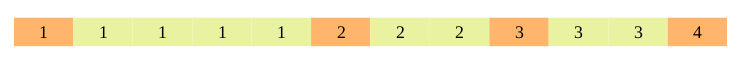
\includegraphics[width=\textwidth]{figures/in_memo}
		\caption{Memory layout}
	\end{figure}
	Connections marked in yellow are right behind their source nodes, marked in orange. 
	This means it is not required storing information about the number and destination addresses 
	of connections because it is enough iterate through memory until it encounters another node 
	that acts as a terminator for the string connections.
	This is similar to the ASCII text string implementation on most systems where the string is 
	represented by a fragment of memory ended with a character with code 0.
\end{frame}

%--------------------------------------------------------------------------------------------------
\begin{frame}
\frametitle{Encoding numerical values}
	\begin{figure}[htb] 
		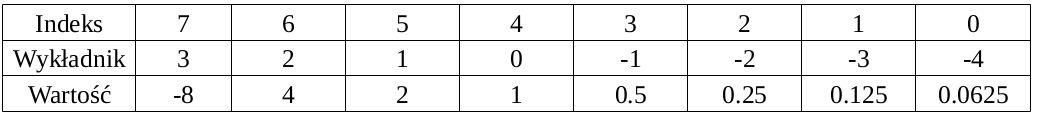
\includegraphics[width=\textwidth]{figures/u2_example}
		\caption{Example of encoding}
	\end{figure}
	Table 2 illustrates the method of encoding the eight-bit number in the fixed-position U2 code,
	the problem of the lack of symmetry in the above encoding becomes immediately apparent.
	The smallest number that we are able to encode is yin = 100000002 = -8 and the largest is 
	ymax = 011111112 = 7.9375.
	This is a problem because in the neural network model the most desirable encoding range is 
	the symmetric interval <-1.1>. 
\end{frame}

%--------------------------------------------------------------------------------------------------
\begin{frame}
\frametitle{Modeling signal}
The second important feature that can be used is the low ratio of active neurons to
the total number of them in the case of larger networks.
Since we expect the generated networks will be of significant size, we can take advantage of this
fact and separate the information about activation nodes from their models to external objects. 
\end{frame}
\end{document}
